% This is a Basic Assignment Paper but with like Code and stuff allowed in it. 

\documentclass[11pt]{article}
% Preamble

\usepackage[margin=1in]{geometry}
\usepackage{amsfonts, amsmath, amssymb}
\usepackage{fancyhdr, float, graphicx}
\usepackage[utf8]{inputenc} % Required for inputting international characters
\usepackage[T1]{fontenc} % Output font encoding for international characters
\usepackage{fouriernc} % Use the New Century Schoolbook font
\usepackage[nottoc, notlot, notlof]{tocbibind}
\usepackage{listings}
\usepackage{xcolor}Problem_B_output

\definecolor{codegreen}{rgb}{0,0.6,0}
\definecolor{codegray}{rgb}{0.5,0.5,0.5}
\definecolor{codepurple}{rgb}{0.58,0,0.82}
\definecolor{backcolour}{rgb}{0.95,0.95,0.92}

\lstdefinestyle{mystyle}{
    backgroundcolor=\color{backcolour},   
    commentstyle=\color{codegreen},
    keywordstyle=\color{magenta},
    numberstyle=\tiny\color{codegray},
    stringstyle=\color{codepurple},
    basicstyle=\ttfamily\footnotesize,
    breakatwhitespace=false,         
    breaklines=true,                 
    captionpos=b,                    
    keepspaces=true,                 
    numbers=left,                    
    numbersep=5pt,                  
    showspaces=false,                
    showstringspaces=false,
    showtabs=false,                  
    tabsize=2
}

\lstset{style=mystyle}

% Header and Footer
\pagestyle{fancy}
\fancyhead{}
\fancyfoot{}
\fancyhead[L]{\textit{\Large{OOPJC Assignment 9}}}
%\fancyhead[R]{\textit{something}}
\fancyfoot[C]{\thepage}
\renewcommand{\footrulewidth}{1pt}



% Other Doc Editing
% \parindent 0ex
%\renewcommand{\baselinestretch}{1.5}

\begin{document}

\begin{titlepage}
	\centering

	%---------------------------NAMES-------------------------------

	\huge\textsc{
		MIT World Peace University
	}\\

	\vspace{0.75\baselineskip} % space after Uni Name

	\LARGE{
		Object Oriented Programming with Java and C++\\
		Second Year B. Tech, Semester 1
	}

	\vfill % space after Sub Name

	%--------------------------TITLE-------------------------------

	\rule{\textwidth}{1.6pt}\vspace*{-\baselineskip}\vspace*{2pt}
	\rule{\textwidth}{0.6pt}
	\vspace{0.75\baselineskip} % Whitespace above the title



	\huge{\textsc{
			Applet Using Java and HTML
		}} \\



	\vspace{0.5\baselineskip} % Whitespace below the title
	\rule{\textwidth}{0.6pt}\vspace*{-\baselineskip}\vspace*{2.8pt}
	\rule{\textwidth}{1.6pt}

	\vspace{1\baselineskip} % Whitespace after the title block

	%--------------------------SUBTITLE --------------------------	

	\LARGE\textsc{
		Practical Report\\
		Assignment 9
	} % Subtitle or further description
	\vfill

	%--------------------------AUTHOR-------------------------------

	Prepared By
	\vspace{0.5\baselineskip} % Whitespace before the editors

	\Large{
		Krishnaraj Thadesar \\
		Cyber Security and Forensics\\
		Batch A1, PA 20
	}


	\vspace{0.5\baselineskip} % Whitespace below the editor list
	\today

\end{titlepage}


\tableofcontents
\thispagestyle{empty}
\clearpage


\setcounter{page}{1}

\section{Aim and Objectives}
\subsection*{Aim}
Develop an applet that displays a simple message in centre of the screen
\subsection*{Objectives}
\begin{enumerate}
	\item To understand concept of Java // Krishnaraj Thadesar
	// Batch A1, PA20
	// OOPCJ Assignment 9Applets
	\item To explore features of applets to develop web applications
\end{enumerate}
\section{Problem Statements}
Write a Java applet program that displays a simple message in centre of the screen.

\section{Theory}
\subsection{Introduction to an Applet and its features}
\textit{Java applets were small applications written in the Java programming language, or another programming language that compiles to Java bytecode, and delivered to users in the form of Java bytecode. The user launched the Java applet from a web page, and the applet was then executed within a Java virtual machine (JVM) in a process separate from the web browser itself. A Java applet could appear in a frame of the web page, a new application window, Sun's AppletViewer, or a stand-alone tool for testing applets.}\\

Java applets were introduced in the first version of the Java language, which was released in 1995. Beginning in 2013, major web browsers began to phase out support for the underlying technology applets used to run, with applets becoming completely unable to be run by 2015-2017. Java applets were deprecated by Java 9 in 2017\\

An applet is a Java program that can be embedded into a web page. It runs inside the web browser and works at client side. An applet is embedded in an HTML page using the APPLET or OBJECT tag and hosted on a web server.
Applets are used to make the website more dynamic and entertaining.\\

Here are some important points:
\begin{itemize}
	\item All applets are sub-classes (either directly or indirectly) of java.applet.Applet class.
	\item Applets are not stand-alone programs. Instead, they run within either a web browser or an applet viewer. JDK provides a standard applet viewer tool called applet viewer.
	\item In general, execution of an applet does not begin at main() method.
	\item Output of an applet window is not performed by System.out.println(). Rather it is handled with various AWT methods, such as drawString().
\end{itemize}
\subsection{The Lifecycle of an Applet}
Five methods in the Applet class gives you the framework on which you build any serious applet.
\begin{enumerate}
	\item \textit{init} - This method is intended for whatever initialization is needed for your applet. It is called after the param tags inside the applet tag have been processed.

	\item \textit{start} - This method is automatically called after the browser calls the init method. It is also called whenever the user returns to the page containing the applet after having gone off to other pages.

	\item \textit{stop} - This method is automatically called when the user moves off the page on which the applet sits. It can, therefore, be called repeatedly in the same applet.

	\item \textit{destroy} - This method is only called when the browser shuts down normally. Because applets are meant to live on an HTML page, you should not normally leave resources behind after a user leaves the page that contains the applet.

	\item \textit{paint} - Invoked immediately after the start() method, and also any time the applet needs to repaint itself in the browser. The paint() method is actually inherited from the java.awt.
\end{enumerate}

\subsection{Discuss about applet tag and its importance}
\textit{An applet may be invoked by embedding directives in an HTML file and viewing the file through an applet viewer or Java-enabled browser.
	The <applet> tag is the basis for embedding an applet in an HTML file.}
\begin{lstlisting}[language=HTML]
	<!DOCTYPE html>
	<html>
	   <head>
		  <title>HTML applet Tag</title>
	   </head>
	   <body>
		  <applet code = "newClass.class" width = "300" height = "200"></applet>
	   </body>
	</html>
\end{lstlisting}
It is now only supported on Internet Exporer, Firefox, and Safari.
Here is an example using the above attributes in the applet tag.

\begin{lstlisting}[language=HTML]
<!DOCTYPE html>
<html>
  <head>
    <title>HTML applet Tag</title>
  </head>
  <body>
    <applet
      code="Demo.class"
      width="300"
      height="200"
      alt="It is a class"
      align="left"
      name="New Applet"
      title="A Title for the Applet"
      vspace="30px"
    ></applet>
  </body>
</html>

\end{lstlisting}

\subsection{Explain various methods of Applet class with necessary examples.}
\begin{table}[H]
	\begin{tabular}{|l|l|l|}
		\hline
		\textbf{Attribute} & \textbf{Value} & \textbf{Description}                                                                    \\ \hline
		align              & URL            & \textit{Deprecated - Defines the text alignment around the applet}                      \\ \hline
		alt                & URL            & Alternate text to be displayed in case browser does not support applet                  \\ \hline
		archive            & URL            & Applet path when it is stored in a Java Archive ie. jar file                            \\ \hline
		code               & URL            & A URL that points to the class of the applet                                            \\ \hline
		codebase           & URL            & Indicates the base URL of the applet if the code attribute is relative                  \\ \hline
		height             & pixels         & Height to display the applet                                                            \\ \hline
		hspace             & pixels         & \textit{Deprecated - Defines the left and right spacing around the applet}              \\ \hline
		name               & name           & Defines a unique name for the applet                                                    \\ \hline
		object             & name           & Specifies the resource that contains a serialized representation of the applet's state. \\ \hline
		title              & test           & Additional information to be displayed in tool tip of the mouse                         \\ \hline
		vspace             & pixels         & \textit{Deprecated - Amount of white space to be inserted above and below the object.}  \\ \hline
		width              & pixels         & Width to display the applet.                                                            \\ \hline
	\end{tabular}
\end{table}

\section{Platform}
\textbf{Operating System}: Arch Linux x86-64 \\
\textbf{IDEs or Text Editors Used}: Visual Studio Code\\
\textbf{Compilers} : g++ and gcc on linux for C++, and javac, with JDK 18.0.2 for Java\\

\section{Output}
The Applet with some text written on it being displayed on the screen.
\begin{figure}[H]
	\centering
	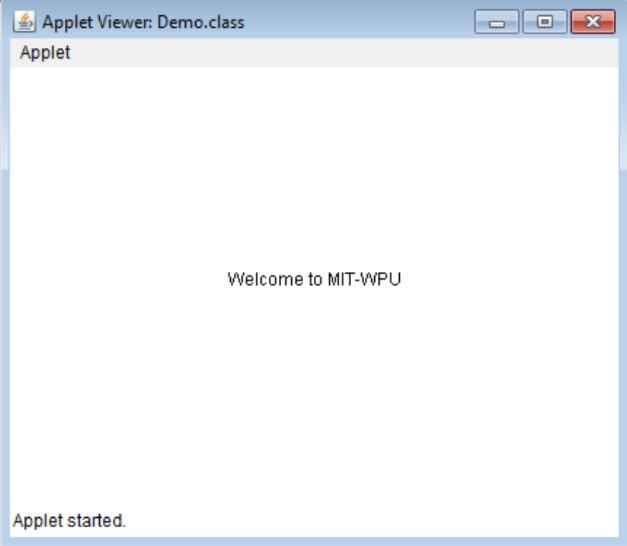
\includegraphics[scale=0.55]{applet.png}
	\caption{}
\end{figure}

\section{Code}

\lstinputlisting[language=java, caption=applet.java]{../Programs/java_implementations/assignment_9/assignment_9.java}
\lstinputlisting[language=html, caption=applet.html]{../Programs/java_implementations/assignment_9/assignment_9.html}

\section{Conclusion}
Thus, developed an applet that displays a simple message in centre of the screen.

% \pagebreakpagebreak

\section{FAQs}
\begin{enumerate}
	\item \textit{What are the restrictions imposed on Java applets?}
	      Mostly due to security reasons, the following restrictions are imposed on Java applets:

	      \begin{enumerate}
		      \item An applet cannot load libraries or define native methods.
		      \item An applet cannot ordinarily read or write files on the execution host.
		      \item An applet cannot read certain system properties.
		      \item An applet cannot make network connections except to the host that it came from.
		      \item An applet cannot start any program on the host that's executing it.
		      \item
	      \end{enumerate}
	\item \textit{What is the applet class loader, and what does it provide?}

	      \textit{The class loader is the means by which Java classes and resources are loaded into the JRE. It controls the policies ranging from where to load class definitions to the data format of the class definitions.}

	      A system class loader responsible for loading in the Java runtime, the application, and classes and resources in the application's classpath. An applet class loader is responsible for loading the applets and their related classes and resources, possibly over the network by communicating with a Web serve

	      When an applet is loaded over the internet, the applet is loaded by the applet classloader. The class loader enforces the Java name space hierarchy. Also, the class loader guarantees that a unique namespace exists for classes that come from the local file system, and that a unique namespace exists for each network source.\\

	      When a browser loads an applet over the net, that applet's classes are placed in a private namespace associated with the applet's origin. Then, those classes loaded by the class loader are passed through the verifier.

	\item \textit{What is the applet security manager, and what does it provide?}
	      A security manager is an object that defines a security policy for an application. This policy specifies actions that are unsafe or sensitive. Any actions not allowed by the security policy cause a SecurityException to be thrown. An application can also query its security manager to discover which actions are allowed.\\

	      Typically, a web applet runs with a security manager provided by the browser or Java Web Start plugin. Other kinds of applications normally run without a security manager, unless the application itself defines one. If no security manager is present, the application has no security policy and acts without restrictions.
	\item \textit{Explain the following with suitable examples}
	      \begin{enumerate}
		      \item \textbf{Creating an applet}
		            \begin{lstlisting}[language=Java]
import java.applet.*;
import java.awt.*;

public class Assignment_9 extends Applet {
    public void print(Graphics g) {
        g.drawString("Welcome to Java Applets in Assignment 9", 150, 150);
    }
}
			  \end{lstlisting}
		      \item \textbf{Passing parameters to applets}
		            \begin{lstlisting}[language=Java]
import java.applet.Applet;  
import java.awt.Graphics;  

public class UseParam extends Applet{  
  
	public void paint(Graphics g){  
	String str=getParameter("msg");  
	g.drawString(str,50, 50);  
	}  
	
}  
\end{lstlisting}
		            \begin{lstlisting}[language=html]
<html>  
<body>  
<applet code="UseParam.class" width="300" height="300">  
<param name="msg" value="Welcome to applet">  
</applet>  
</body>  
</html>  
\end{lstlisting}
		      \item \textbf{Adding graphics and colors to applets.}
		            \begin{lstlisting}[language=Java]
import java.applet.Applet;  
import java.awt.*;  

public class GraphicsDemo extends Applet{  

	public void paint(Graphics g){  
		g.setColor(Color.red);  
		g.drawString("Welcome",50, 50);  
		g.drawLine(20,30,20,300);  
		g.drawRect(70,100,30,30);  
		g.fillRect(170,100,30,30);  
		g.drawOval(70,200,30,30);  

		g.setColor(Color.pink);  
		g.fillOval(170,200,30,30);  
		g.drawArc(90,150,30,30,30,270);  
		g.fillArc(270,150,30,30,0,180);  
	}  
} 
				\end{lstlisting}
		            \begin{lstlisting}[language=html]
<html>  
<body>  
<applet code="GraphicsDemo.class" width="300" height="300">  
</applet>  
</body>  
</html>  
				\end{lstlisting}
	      \end{enumerate}
\end{enumerate}
\end{document}